\documentclass[twocolumn,
			   showpacs,%
               nofootinbib,
               aps,%
               %eqsecnum,
               prd,
               notitlepage,
               showkeys,
               10pt]{revtex4-1}
               
%Loading my personal settings
\usepackage{todonotes}

%math and formulas
\usepackage{amssymb}
\usepackage{amsmath}
\usepackage{physics}

%language settings and microtype
\usepackage[english]{babel}
\usepackage{microtype}

%useful packages
\usepackage{graphicx}
\usepackage{siunitx}
\usepackage{xcolor}
\usepackage{float}
\usepackage{dcolumn}
\usepackage{blindtext}
\usepackage{xfrac}
\usepackage[labelfont=bf]{caption}
\usepackage{subcaption}


%feynman diagrams
\usepackage{tikz}
\usepackage{tikz-feynman}
\tikzfeynmanset{compat=1.0.0} 

%loading the `external` library
\usetikzlibrary{external}   
%Create directory to store the diagrams and all related files          
\immediate\write18{mkdir -p feynman-diagrams} 
% Activate externalization
\tikzexternalize[
  %Avoid cluttering the directory                     
  prefix=feynman-diagrams/, 
  %Calling lualatex externally
  system call={             
    lualatex \tikzexternalcheckshellescape -halt-on-error -interaction=batchmode -jobname="\image" "\texsource"  || rm "\image.pdf"
  },
]

%color settings
\definecolor{mydarkblue}{RGB}{1,1,141}

%correcting parindent
\setlength{\parindent}{0pt}


%always use hyperref at the end of the preamble!
\usepackage[colorlinks=True]{hyperref}
\hypersetup{allcolors=mydarkblue}
%main document
\begin{document}

%Personel data
{\hypersetup{allcolors=black}
\title{F91: Studying the $Z$ boson with the ATLAS Detector at the LHC }
\author{Mathieu Kaltschmidt}
\email{M.Kaltschmidt@stud.uni-heidelberg.de}
\affiliation{Heidelberg University,  D-69117 Heidelberg, Germany}
\author{Quirinus Schwarzenb\"ock}
\email{Schwarzenb\"ock@stud.uni-heidelberg.de}
\affiliation{Heidelberg University,  D-69117 Heidelberg, Germany}

\date[Carried out in the week of  ]{March 4$^{\text{th}}$, 2019}


\begin{abstract}
This experiment was performed as part of the advanced lab course for physics students (FP) at Heidelberg University.
The goal of this computer-based experiment is to determine the invariant mass spectrum of the $Z$ boson, one of the three massive gauge bosons of the weak interaction, for decays into $e^+e^-$-, $\mu^+\mu^-$- and $\tau^+\tau^-$-pairs. We use data acquired by the ATLAS experiment at the Large Hadron Collider (LHC) at CERN in Geneva at a center-of-mass energy of $\sqrt{s} = 8 $ TeV and with an integrated luminosity of $\mathcal{L}_{\text{int}} = 1 \ \text{fb}^{-1}$. An event selection is performed to distinguish between signal and background events. We find a $Z$ mass of $M_{\mathrm{Z}} = (90.607 \pm 0.004)$ GeV with a decay width of $\Gamma = (3.517 \pm 0.015)$ GeV and a standard deviation of $\sigma = (1.559 \pm 0.015)$ GeV.
\end{abstract}

\maketitle


}
\section{Introduction}
In this lab course we want to study the properties of the $Z$ boson and get familiar with modern data analysis tools such as \verb|ROOT| and \verb|Python3|, used in current experimental high-energy physics research. The data we analyzed is part of the ATLAS Open Data set \cite{DATA}, published by CERN to provide students a hands-on training experience for data analysis. It features data from the LHC measured in 2012 and additionally some Monte Carlo simulations of the same decay channels ($Z\rightarrow e^+e^-,Z\rightarrow \mu^+\mu^-$ and $Z\rightarrow \tau^+\tau^-$) for a better comparability with the theoretical predictions.

\subsection{The $Z$ boson}
In this section, we want to introduce the theoretical properties of the $Z$ boson. The most important ones are summarized in table (\ref{tab:Z_props}).

\begin{table}[!htbp]
	\centering
	\renewcommand{\arraystretch}{1.5}
	\begin{tabular}{c|c|c|c}
	Charge $Q$ & Spin $S$ & Mass $M_Z$ [GeV] & Decay Width $\Gamma$ [GeV] \\ \hline 
	 0 & 1 & $(91.1876 \pm 0.0021)$ & $(2.4952 \pm 0.0023)$ \\
		\end{tabular}
	\caption{\label{tab:Z_props}The properties of the $Z$ boson.}
	\label{tab:Z_props}
\end{table}

The $Z$ boson is one of the three gauge bosons of the weak interaction. In contrast to photons, which mediate the electromagnetic force, or gluons, the gauge bosons of the strong interaction, it is massive. It has two charged "cousins", the $W^+$ and the $W^-$ boson. Postulated by Glashow, Salam and Weinberg in the 1960s as part of the unified electroweak interaction, which earned them a Nobel prize in 1979, it has not been directly observed until 1983, at the SPS collider at CERN, when particle colliders were able to reach center-of-mass energies high enough. The detection of the $Z$ boson earned Carlo Rubbia and Simon van der Meer also a Nobel prize in 1984 \cite{F91manual}.   


\section{Theoretical Foundations}
This section introduces the basic knowledge on particle and detector physics needed for a general understanding of the conducted experiment.

\subsection{Drell-Yan Processes}
At the LHC, hadrons, i.\,e. particles made up of three quarks, scatter at very high energies. An important role in these collision events play Drell-Yan processes. These occur, when a quark and its corresponding antiquark annihilate each other via a virtual boson, for example a $Z$, which we are interested in in this lab course. A Feynman diagram for an example of a Drell-Yan process is depicted in the following in figure (\ref{fig:Drell-Yan}).

\begin{figure}[H]
\centering
\feynmandiagram [small] [horizontal' = a to b] {
	i1 [particle=\(q\)] -- [fermion] a  -- [fermion] i2 [particle=\(\overline{q}\)],
	a -- [photon, edge label=\(\gamma / Z^0\)] b ,
	f1 [particle=\(l^{+}\)] -- [fermion] b -- [fermion] f2 [particle=\(l^{-}\)],
	};
\caption{A tree-level Drell-Yan diagram \cite{F91manual}.}
\label{fig:Drell-Yan}
\end{figure}
	
To study the properties of the gauge bosons involved in these processes one can calculate for example the invariant mass $\sqrt{s}$, using the following formula:
\begin{align}
	\sqrt{s} = \sqrt{\left(p_{l^{-}} + p_{l^{+}}\right)^2}
\end{align}
We will see later on, how this formula can be used to distinguish between data and background.
\subsection{Characteristics of Particle Detectors}
In circular particle colliders such as the LHC, two opposed proton beams, each containing $n_b = 1380$ bunches with approximately $N_i = 10^{11}$ protons are accelerated to almost the speed of light and forced to collide at very high center-of-mass energies, e.\,g. $\sqrt{s} = 8$ TeV in the first run of the LHC. An important characteristic of circular colliders is the \textit{luminosity} $\mathcal{L}$, given by

\begin{align}
\mathcal{L} = \frac{N_1N_2f_{\text{rev}}n_b}{4\pi\sigma_x\sigma_y},
\end{align}
where $f = 11.2$ kHz describes the orbital frequency of the beams and the $\sigma_i$ describe the smearing of the beam in the respective direction. At Run 2 of the LHC, luminosities of $\mathcal{L}=2\cdot10^{34} \ \mathrm{cm}^{-2} \mathrm{s}^{-1}$ are reached.\\
Another interesting quantity is the \textit{integrated luminosity}, the luminosity integrated over time:
\begin{align}
\mathcal{L}_{\text{int}} = \int \mathcal{L} \ \dd t.
\end{align}
The data we are analyzing has an integrated luminosity of $\mathcal{L}_{\mathrm{int}}=1 \ \mathrm{fb}^{-1}$.\\
Together with the \textit{total cross section} $\sigma_{pp\rightarrow X}$ one finds the following relation for the total number of events $N$: 
\begin{align}
N = \sigma_{pp\rightarrow X} \cdot \mathcal{L}_{\text{int}}.
\end{align}

\subsection{Energy distributions}
\textbf{Gaussian distribution.} Inside the calorimeter, the energies are distributed following a \textit{Gaussian}, i.\,e. 
\begin{align}
g(E ; \mu, \sigma)=\frac{\mathcal{N}}{\sqrt{2 \pi} \sigma} \exp \left[-\frac{(E-\mu)^{2}}{2 \sigma^{2}}\right],
\label{eqn:Gaussian}
\end{align}
with an normalization constant $\mathcal{N}$, representing the event number. The important parameter in this distribution is the standard deviation $\sigma$ which allows us to estimate the uncertainty of the energy.\\

\textbf{Breit-Wigner distribution.} The physical decay process is described by the \textit{Relativistic Breit-Wigner distribution}, 
\begin{align}
	f(E ; M, \Gamma)=\frac{\mathcal{N} k}{\left(E^{2}-M^{2}\right)^{2}+M^{2} \Gamma^{2}},
\end{align}
where $k=\frac{2 \sqrt{2} M \Gamma \gamma}{\pi \sqrt{M^{2}+\gamma}}$ and $\gamma=M \sqrt{M^{2}+\Gamma^{2}}$. The parameter $M$ represents the mass and $\Gamma$ is the decay width of the observed process. For a derivation see for example \cite{BohmSato2004}. \\

In order to describe the real measured process we have to convolute a Breit-Wigner distribution and a Gaussian. This takes the smearing of the curve due to the finite energy resolution into account, which is described by the Gaussian (\ref{eqn:Gaussian}). \\

The convolution of both distributions leads us to the so called \textit{Relativistic Voigt Profile}
\begin{align}
	V(E ; M, \Gamma, \sigma)=\int \mathrm{d} E^{\prime} g\left(E^{\prime} ; 0, \sigma\right) f\left(E-E^{\prime} ; M, \Gamma\right).
\end{align}
We will use this function later on to fit the filtered data set. A comparison to the fit with the two single distributions is also included. 
\subsection{The ATLAS Detector at the LHC}

Three major components form the setup of the ATLAS detector, i.\,e. the \textit{Inner Detector}, which aims at reconstructing the tracks of charged particles passing the detector, the \textit{Calorimeter}, where the electromagnetic and hadronic showers are evaluated and the \textit{Muon Spectrometer} in the outer layer, to reconstruct muon tracks, which have in general a free path length much longer than the other charged particles occurring in $pp$-collisions. Additionally, there is a complex \textit{Trigger System} to avoid the collection of irrelevant data and the so called \textit{GRID}, a network to make the measured data accessible to the world-wide particle physics community working on ATLAS physics. \\
A schematic overview is presented in figure (\ref{fig:atlas}) in the following.
\begin{figure}[H]
\centering
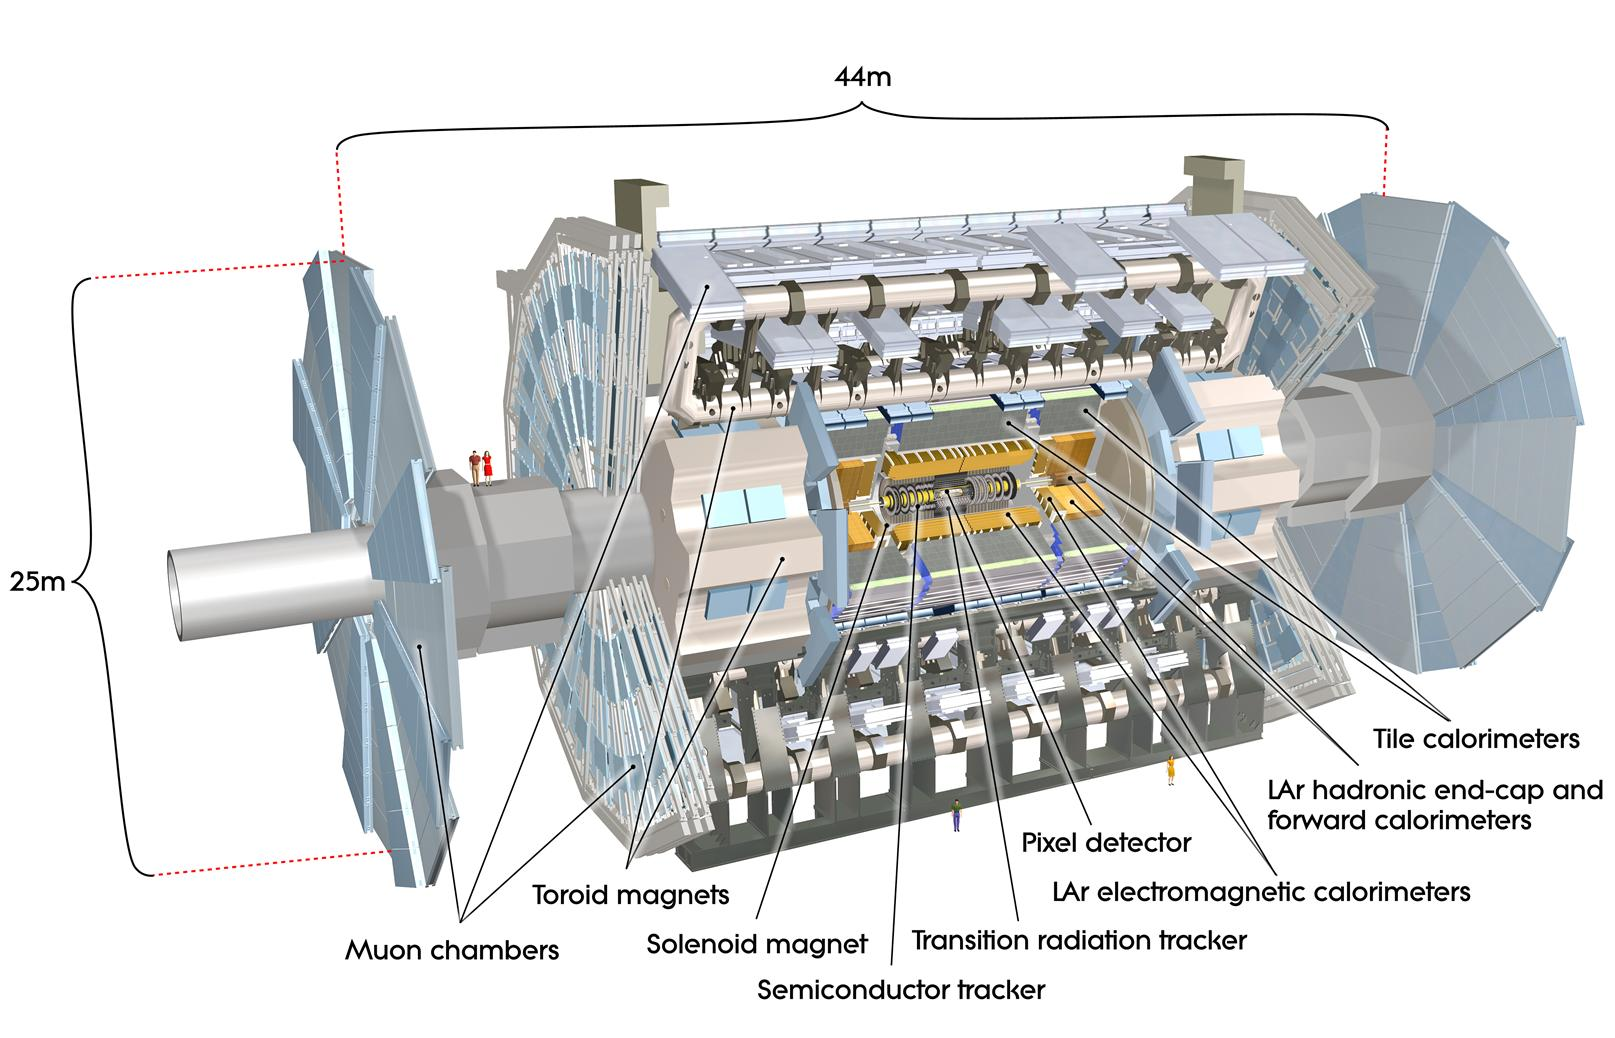
\includegraphics[width=0.45\textwidth]{figures/introduction/atlas}
\caption[Schematic picture of the ATLAS detector at the LHC.]{Schematic picture of the ATLAS detector at the Large Hadron Collider \cite{ATLAS}.}
\label{fig:atlas}
\end{figure}

\subsection{Detector Geometry}
An important quantity for the understanding of the geometry of particle detectors is the \textit{pseudorapidity} $\eta$, which is used to describe polar angle distributions, i.\,e.
\begin{align}
\eta = -\ln \tan(\frac{\theta}{2}).	\label{eqn:eta}
\end{align}

From the geometry of the setup we find the following relations between the momentum components $p_i$ and the transversal momentum $p_T$:
\begin{align}
	p_x &= p_T \cos(\phi)\\
	p_y &= p_T \sin(\phi)\\
	p_z \tan(\theta) &= p_T
\end{align}
From equation (\ref{eqn:eta}) and by using the identity
\begin{align*}
\tan(2\arctan(x)) = \frac{2x}{1 - x^2},
\end{align*} 
we arrive at the following equations:
\begin{align}
	p_z &= p_T\sinh(\eta)\\
	\left|\mathbf{p}\right| &= p_T \cosh(\eta).
\end{align}


\subsection{Efficiency of the $e^-$ detection.}
This section describes the so called \textit{tag and probe method}, which allows us to determine the unbiased efficiency of the measurement and filtering process.\\
One of the two electrons (the \textit{tag} electron) has to pass very strong selection criteria. The next step is to check whether the second electron (the \textit{probe} electron) passes less strict criteria, which are explained in more detail later on, when we discuss the implementation of the multi-level filter system. \\
Then, the last step is to determine the efficiency $\epsilon$ by calculating the ratio between the successful passing probe electrons and the total number of probes.\\
For the \textit{total efficiency} $\epsilon_{\text{tot}}$ we find 
\begin{align}
	\epsilon_{\text{tot}} = \epsilon_{\text{reconstr.}} \cdot \epsilon_{\text{ident.}} \cdot \epsilon_{\text{trigger}} \cdot \epsilon_{\text{add.}}.
\end{align}

\section{Experiment}

Having to learn the basics of \verb|ROOT| and to get familiar with the dataset, we start with the analysis of plots giving us already information about the most important characteristics of the conducted measurements.\\

\textbf{Primary Vertices.} First we have a look at the distribution of the primary vertices along the $z$-axis after a collision of two bunches.\\
The observed Poissonian distribution is explained by the fact, that the bunches are spread along the $z$-axis, which makes it impossible for all collisions to happen at the same $z$-coordinate.\\

\textbf{Lepton Number.} It is possible for two-quark decay-processes to end up in one-, two- or three-lepton final states. \footnote{Neutrinos are neglected in this consideration, since they are very hard to detect.} The following Feynman diagrams represent some of the constellations mentioned above. 

\begin{figure}[H]
\centering	
\feynmandiagram [small] [horizontal' = a to b] {
	i1 [particle=\(\overline{u}\)] -- [fermion] a  -- [fermion] i2 [particle=\(d\)],
	a -- [photon, edge label=\(W^{-}\)] b ,
	f1 [particle=\(\overline{\nu}_{e^{-}}\)] -- [fermion] b -- [fermion] f2 [particle=\(e^{-}\)],
	};
\caption{1-Lepton final state.}
\end{figure}

\begin{figure}[H]
\centering	
\feynmandiagram [small] [horizontal' = a to b] {
	i1 [particle=\(q\)] -- [fermion] a  -- [fermion] i2 [particle=\(\overline{q}\)],
	a -- [photon, edge label=\(\gamma / Z^0\)] b ,
	f1 [particle=\(e^{+}\)] -- [fermion] b -- [fermion] f2 [particle=\(e^{-}\)],
	};
\caption{2-Lepton final state.}
\end{figure}

\begin{figure}[H]
\centering	
\begin{tikzpicture}
  \begin{feynman}
    \vertex (a) {\(d\)};
    \vertex [right=of a] (b);
    \vertex [above right=of b] (c);
    \vertex [above right=of c] (f1) {\(e^{-}\)};
    \vertex [below right=of c] (f2) {\(\overline{\nu}_{e^{-}}\)};
    \vertex [below =of a] (d) {\(\overline{u}\)};
    \vertex [right=of d] (e);
    \vertex [below right=of e] (f);
     \vertex [above right=of f] (f3) {\(e^{-}\)};
    \vertex [below right=of f] (f4) {\(e^{+}\)};

 
    \diagram* {
      (a) -- [fermion] (b) -- [boson, edge label=\(W^{-}\)] (c),
      (d) -- [anti fermion] (e) -- [boson, edge label'=\(Z^{0}\)] (f),
      (f1) -- [anti fermion] (c) -- [anti fermion] (f2),
      (f3) -- [anti fermion] (f) -- [anti fermion] (f4),
      
      (b) -- [edge label' = \(\overline{u}\) ] (e),
};
  \end{feynman}
\end{tikzpicture}
\caption{3-Lepton final state.}
\end{figure}

To check this, we plotted the amount of lepton candidates in the final state for our dataset. The result is presented in the following in figure (\ref{fig:lep_n}).

\begin{figure}[H]
	\centering
	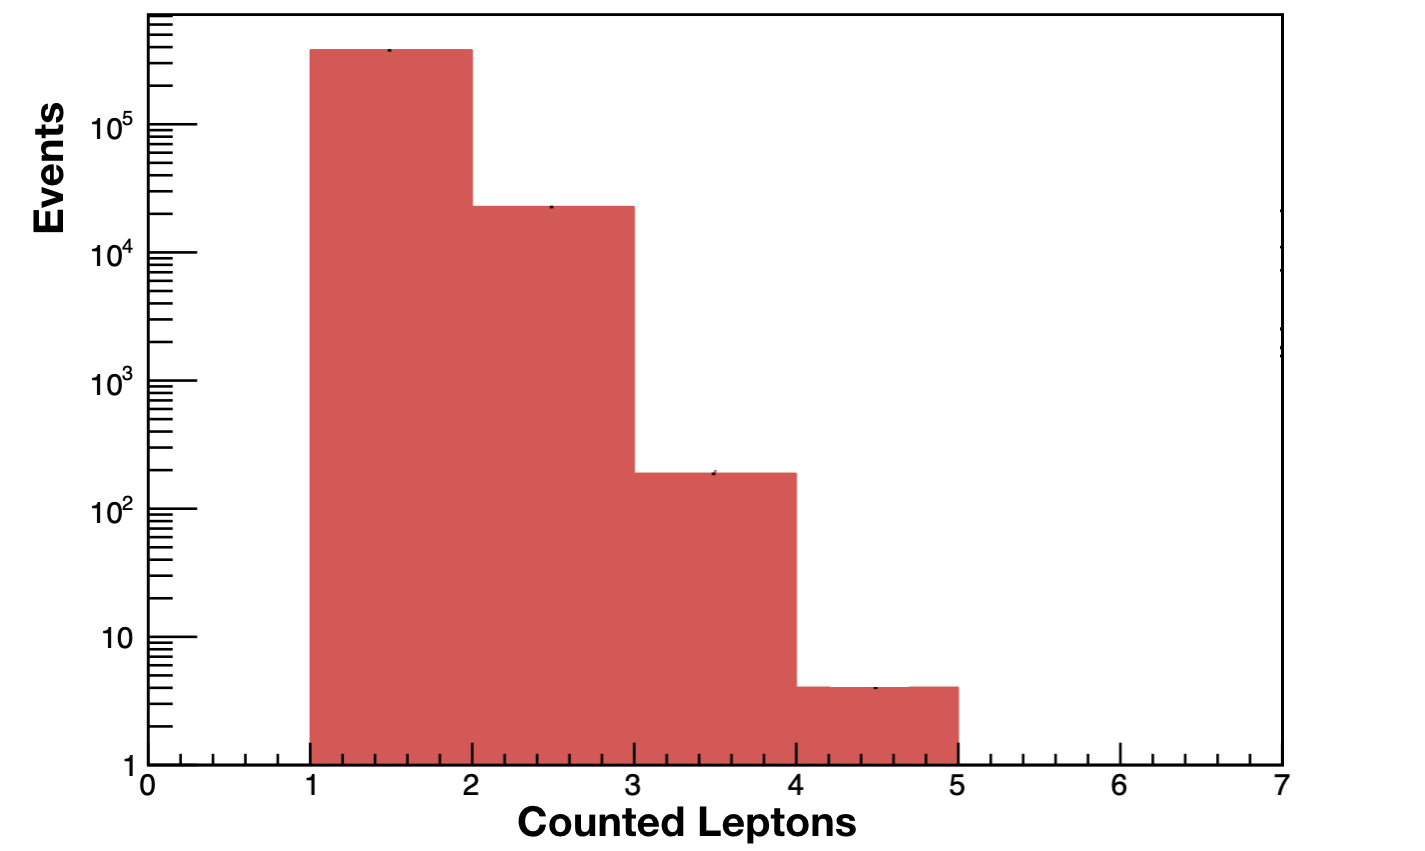
\includegraphics[width=0.45\textwidth]{figures/plots/lep_n_corr}
	\caption{Number of Leptons in the final state.}
	\label{fig:lep_n}
\end{figure}
%TODO: Fix this plot..
There are no $Z$ bosons involved in the 1-lepton final state and in leading order one would expect two leptons in the final state of the decay process. We are going to take this into account, when setting up our filters.\\

\textbf{Angular and Momentum Distributions.}  
Next we take a look at the distribution of  the pseudorapidity $\eta$, the transversal momentum $p_T$ and the azimutal angle distribution $\phi$.

We would expect, by construction, homogeneously distributed dependencies, but this is only true for $\phi$, while for $\eta$ there are obvious deviations from this.
These can  be explained by the geometry of the sub-detector, an explanation that is supported by the symmetry of the stated deviations.\\

The distribution of the transversal momentum depicted in figure (\ref{fig:p_t}), shows an unexpected step at about $20$ GeV, caused by the trigger which sorts out all the events where not at least one Lepton has an energy higher than $25$ GeV\footnote{This is useful since it is very unlikely that these events contain a Z boson candidate.}.
\begin{figure}[H]
	\centering
	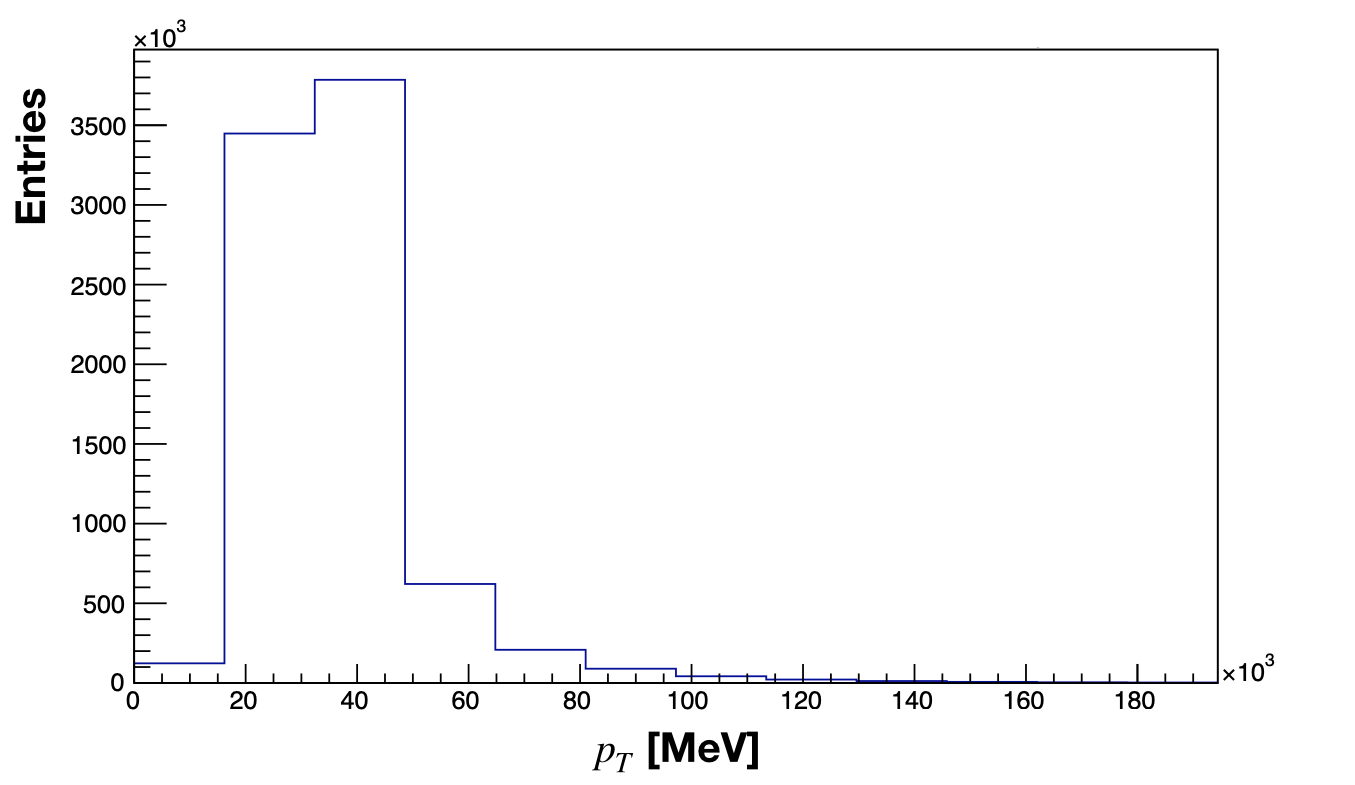
\includegraphics[width=0.45\textwidth]{figures/plots/TransverseMomentum_corr}
	\caption{Distribution of the transverse momentum $p_T$.}
	\label{fig:p_t}
\end{figure}
%TODO: Fix the y-axis
\subsection{Automating things}
For the next part we adapted the already partially implemented \verb|python| script \verb|eventloop.py| to our needs. New functions for calculating the invariant mass of the two leading leptons, using \verb|ROOT|'s inbuilt function \verb|TLorenzVector| on the one hand and the theoretical formula $M = \sqrt{E_0^2 - \mathbf{p}^2}$ for the invariant mass on the other hand, are defined. A comparison of both approaches did only show negligible differences that are probably due to truncation errors.\\

Plotting the distribution of the invariant masses in our dataset we could identify several peaks. Their cause is noted on the adjacent plot.
\begin{figure}[H]
	\centering
	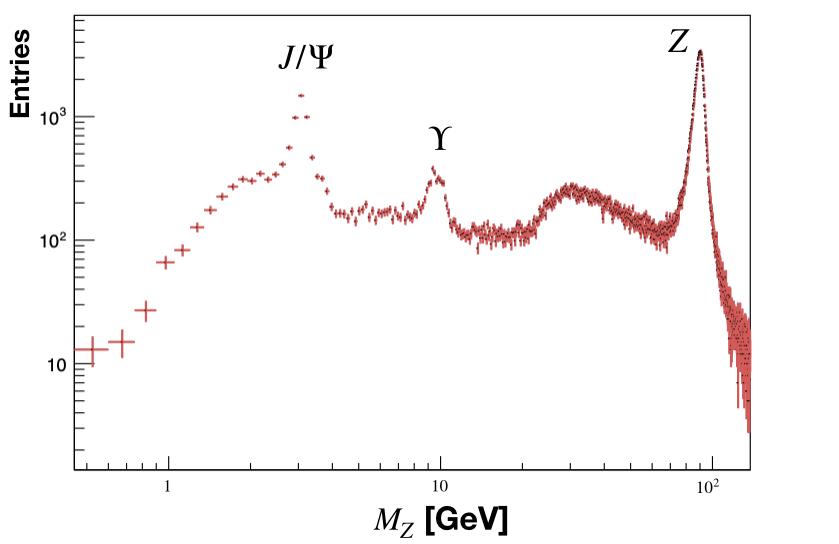
\includegraphics[width=0.45\textwidth]{figures/plots/MassDist_Data_corr}
	\caption{Unfiltered spectrum of the invariant mass distribution for the real dataset.}
\end{figure}

One can clearly see the peak at about $90$ GeV, representing the $Z$ boson. There are some other peaks visible in the data, one at $\sim 3$ GeV and the other at $\sim 10$ GeV which correspond to $J/\Psi$ and $\Upsilon$ meson decays. That is the reason why we can't observe such peaks in the Monte Carlo simulation. As already mentioned before, there is a peak-like structure at around $25$ GeV due to the internal trigger threshold.

\subsection{Selecting events}
To aim for the best possible results, in this part we implemented a series of filters, only leaving the decay processes we could confidently connect to the decay of a Z boson.
The following filters were used:
\begin{enumerate}
\item \textbf{Weigths} (for Monte Carlo simulations only): Normalization factors for the respective simulation.
\item \textbf{Trigger}: Criteria judging whether it is likely for an event to involve a $Z$ boson decaying into an $e^{+}e^{-}$- or $\mu^{+}\mu^{-}$-pair.
\item \textbf{Vertex}: We check, if there is a comprehensible primary vertex for the event.
\item \textbf{2 Leptons}: We are only interested in including events involving exactly two leptons.

\item \textbf{PDGID}: This filter is based on the track reconstruction in the detector, which results in an either \textit{loose, medium} or \textit{tight} prediction of the particle type. Every particle type is identified by an integer number (e.\,g. $e = 11 , \ \mu = 13$ and $\tau = 15$).
\item \textbf{$p_T$ Cut}: A threshold of $p_{T,\text{min}} = 25$ GeV is implemented to make sure that the leptons have an energy high enough to possibly originate from a $Z$ boson decay.

\item \textbf{Isolation}: The relative isolation of $E_T$ and $p_T$ are analyzed by computing the ratio between the amount of energy/momentum inside a cone with a radius of 0.3 respectively 0.2 and the measured energy/momentum. Only ratios smaller than 0.1 pass this step. This filter is applied to separate the lepton candidates we are interested in from those produced in QCD background processes involving jets.  

\item \textbf{Tight ID}: Only the particles labelled as \textit{tight} are considered for further analysis.
\item \textbf{$Z$ Mass}: Checking wether the calculated invariant mass is anywhere near the theoretical invariant mass of a $Z$ boson. Only events with masses between $70$ GeV $ \leq M_Z \leq$  $110$ GeV pass this filter.
\end{enumerate}

After applying all the filters to the data we could plot the number of events that passed the tests up to a certain  filter. This kind of diagram is called \textit{Cut Flow diagram}. For our filter setting, the Cut Flow diagram is depicted in the following.

\begin{figure}[H]
\centering
\includegraphics[width = 0.5\textwidth]
{figures/plots/CutFlowEGamma_corr}
\caption{Cut flow diagram for our event selection algorithm applied to the $Z\rightarrow e^+e^-$ dataset.}	
\end{figure}
As one can clearly see, the most data is discarded after testing if there are exactly 2 Lepton candidates detected in an event. This is in accordance with the result from figure (\ref{fig:lep_n})

In order to be able to compare the data to the theoretical predictions, we analyze Monte Carlo simulations of $Z$ boson decays into $e^+e^-$-, $\mu^+\mu^-$- and $\tau^+\tau^-$-pairs. \\
For a more realistic comparison, we need to rescale the normalization of the simulation to match it to the expected number of events given $\mathcal{L}_{\text{int}}$. We use the formula $k = \sfrac{\mathcal{L}_{\text{int}}\sigma}{w}$, where $w$ represents the MC weight we introduced above. In practice, the scaling is fixed directly in the \verb|Python| script, which means there is no warranty at all that the scaling is set optimally. \\
\begin{figure}[H]
	\centering
	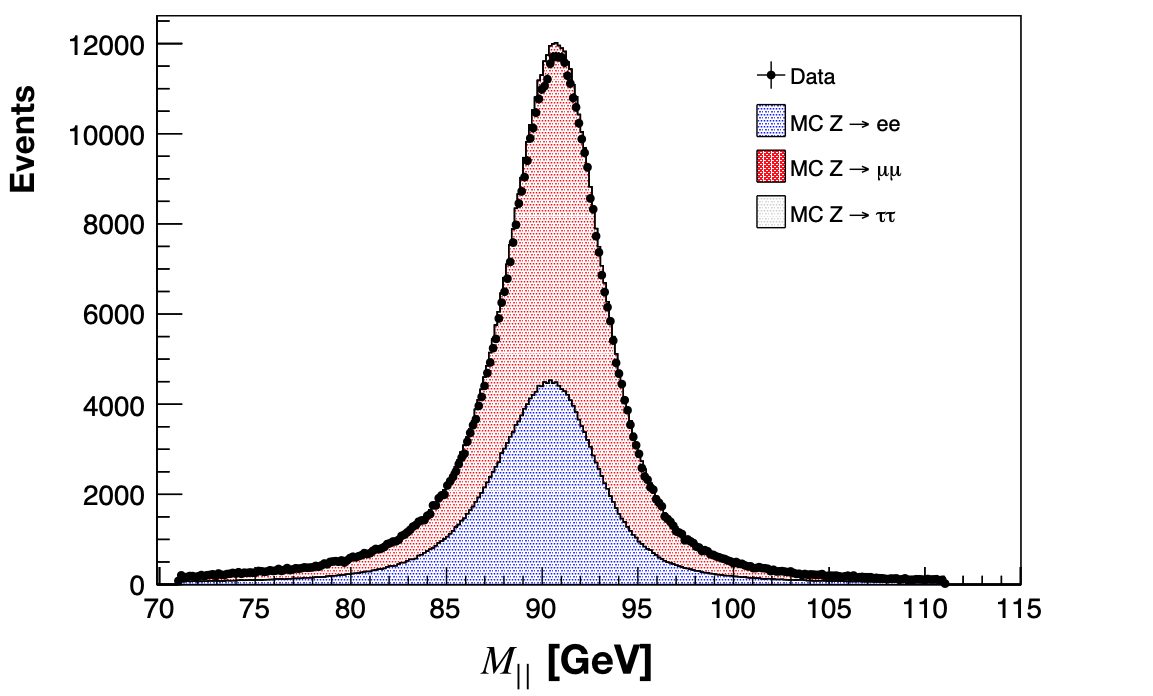
\includegraphics[width=0.45\textwidth]{figures/plots/HistoMCData_corr}
	\caption{Results of the Monte Carlo simulations of $Z$ boson decays into $e^+e^-$-, $\mu^+\mu^-$- and $\tau^+\tau^-$-pairs, compared to the data.}
	\label{fig:MChisto}
\end{figure}
The histogram in figure (\ref{fig:MChisto}) shows that the results from the simulations are in agreement with the data. The $Z\rightarrow \tau^+\tau^-$ peak is almost invisible. This can be explained by the fact, that the $\tau$s usually decay into electrons or muons (and the respective neutrinos + a $\tau$-neutrino) subsequently.

\section{Fitting the $Z$ mass}

We want to use this section to present the final result for the mass distribution of the processes with $Z$ candidates which passed all filter levels. The result is presented in the following in figure (\ref{fig:MassDist}).

\begin{figure}[H]
	\centering
	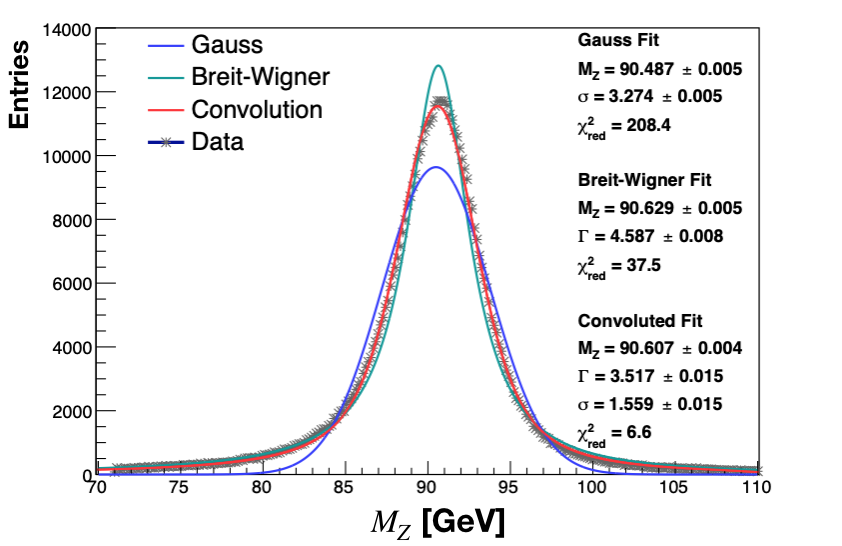
\includegraphics[width = 0.45\textwidth]{figures/plots/ZMass_corr}
	\caption{Distribution of the $Z$ mass $M_{\mathrm{Z}}$ with Gaussian, Breit-Wigner and a convoluted fit.}
	\label{fig:MassDist}
\end{figure}

As discussed before, to obtain a satisfying fitting result, one needs to convolute a Breit-Wigner distribution and a Gaussian. We can directly see in figure (\ref{fig:MassDist}) that the fits using the two functions separately did not represent the physical model in an adequate manner.
The results from the convoluted fit are the following: \\

For the mass of the $Z$ boson we found
\begin{align}
	M_{\mathrm{Z}} = (90.607 \pm 0.004) \ \text{GeV},
\end{align} 
the decay width $\Gamma$ is
\begin{align}
\Gamma = (3.517 \pm 0.015) \ \text{GeV},	
\end{align}
and the Gaussian we used to describe the smearing of the distribution due to the measurement process has a standard deviation of 
\begin{align}
	\sigma = (1.559 \pm 0.015) \ \text{GeV}.
\end{align}

These results can be compared to the values of the Particle Data Group\footnote{The values can be found here: \url{http://pdg.lbl.gov/2018/listings/rpp2018-list-z-boson.pdf}} (PDG), 
\begin{align}
	M_{\mathrm{Z}}&=(91.1876 \pm 0.0021) \ \mathrm{GeV} \\  \nonumber\\ \Gamma&=(2.4952 \pm 0.0023) \ \mathrm{GeV}.
\end{align} 
Using Gaussian error propagation one finds for the differences between our final results and the PDG data
\begin{align}
	\Delta M_{\mathrm{Z}}&=(0.581 \pm 0.005) \ \mathrm{GeV} \\  \nonumber\\ 
	\Delta\Gamma&=(1.022 \pm 0.015) \ \mathrm{GeV},
\end{align} 
which means the deviations are approximately of order $\sim$ 1 GeV. The errors seem to be very small, which is explained by the fact that all errors we take into account only come from the fitting process. This is a highly underestimating treatment of errors.\\

As explained in the introduction, we performed the tag-and-probe method to determine the efficiency of the electron detection for the $Z\rightarrow e^+e^-$ data and for one Monte Carlo simulation. The result is depicted below in figure (\ref{fig:eff}).

\begin{figure}[H]
\centering
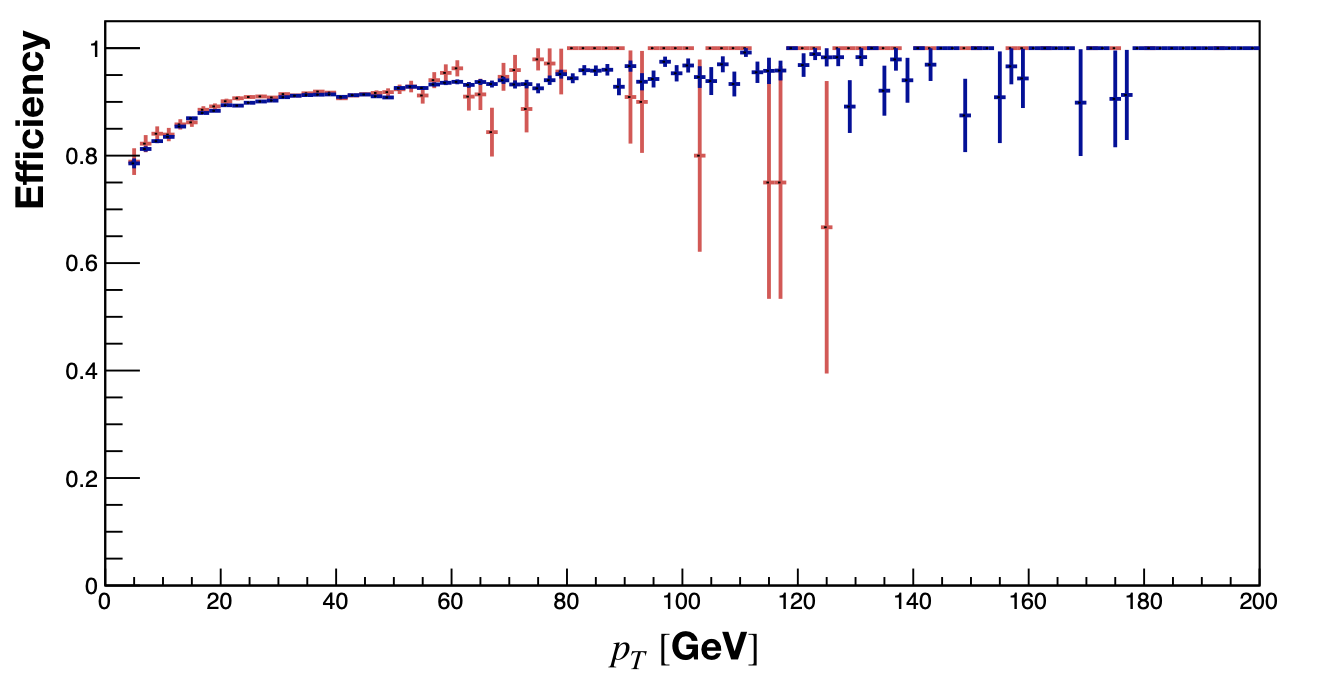
\includegraphics[width=0.45\textwidth]{figures/plots/Efficiency_corr}
\caption{Efficiency measurement for the data (red) and the MC simulation (blue).}
\label{fig:eff}
\end{figure}
We see, that there is a very high efficiency of $\sim$ 0.9 or even higher over almost the entire momentum range.

\section{Critical discussion}
In this section we want to discuss the role of the systematic and statistical errors and their possible influence on our results.\\
The data set we analyzed is sufficiently large, this means we had enough measurements to reduce statistical uncertainties to a negligible minimum. We know from Poisson statistics, that the significance of the corresponding errors can be estimated using the inverse square root of the amount of data. In total this means that it should hold, that $\Delta_{\mathrm{stat.}} \ll \Delta_{\mathrm{syst.}}$. \\
A measure for the possible influence of the systematical uncertainties is given by the standard deviation \\ $\sigma = (1.559 \pm 0.015) \ \text{GeV}$ we extracted from the convoluted fit. It clearly shows that one has to keep in mind that the energy resolution inside the calorimeter is finite and limited. This could hopefully be improved in the future, when the hardware of the detector is updated.  In general one has to think about the threshold values for the filter system. If we would have had additional time, we could have tested the impact of changes in the different steps of the implemented filter. \\
Another way of dealing with possible error sources from various background processes would be to include some Monte Carlo simulations of these processes (e.\,g. for the QCD processes or the decays including $\Upsilon$'s or $J/\Psi$'s we could observe in the mass spectrum), to once again improve the understanding of the different residuals in the recorded data. This could also be helpful for the choice of the limits for the different selection criterions. \\
We can conclude that it is difficult to estimate the errors arising on the one hand from the analysis of the data and on the other hand from the complex processes taking place during such high-energy particle collisions. The better one understands the (sub-)structures of the data, the easier it is to test the results using e.\,g. theoretical predictions via simulations or to find weak spots in the hardware of the detector.

\section{Conclusion}
After some preparation time to be able to understand the underlaying structure of the analyzed dataset, the main goal of this lab course was to get familiar with modern data analysis tools such as \verb|ROOT| and \verb|Python| and to handle a large amount of data by implementing our own multi-level filter system, to be able to distinguish possible $Z$ boson candidates from other background processes. We also had the chance to compare the data to theoretical predictions by analyzing Monte Carlo simulations. Our final result for the $Z$ mass and its decay width $\Gamma$ would probably be in accordance with the values provided by the PDG, if the treatment of errors we mentioned in the last section would be included in our estimations. Nevertheless we can conclude that the obtained results are compatible with the expectations.\\
We also measured the efficiency of the electron detection using the tag and probe method, which allowed us to estimate the systematic errors due to uncertainties in the measure electronics, especially inside the calorimeter.\\
 
\begin{acknowledgments}
We would like to thank our supervisor Philipp Ott for his guidance throughout the operation of this experiment.
\end{acknowledgments}

\bibliographystyle{abbrv}
\bibliography{bibliography/literatur}
\nocite{*}

\end{document}
